% Created 2020-05-21 Thu 14:22
% Intended LaTeX compiler: pdflatex
\documentclass[11pt]{article}
\usepackage[utf8]{inputenc}
\usepackage[T1]{fontenc}
\usepackage{graphicx}
\usepackage{grffile}
\usepackage{longtable}
\usepackage{wrapfig}
\usepackage{rotating}
\usepackage[normalem]{ulem}
\usepackage{amsmath}
\usepackage{textcomp}
\usepackage{amssymb}
\usepackage{capt-of}
\usepackage{hyperref}
\usepackage{minted}
\usepackage{/home/ryan/Dropbox/profiles/Templates/LaTeX/ScreenStyle}
\author{Ryan Greenup}
\date{\today}
\title{Ananlysis of COVID Data}
\hypersetup{
 pdfauthor={Ryan Greenup},
 pdftitle={Ananlysis of COVID Data},
 pdfkeywords={},
 pdfsubject={},
 pdfcreator={Emacs 27.0.91 (Org mode 9.4)}, 
 pdflang={English}}
\begin{document}

\maketitle
\tableofcontents


\section{Preliminary}
\label{sec:org65e16aa}
\subsection{Load Packages and Data}
\label{sec:org32a0c5d}

\begin{minted}[]{r}
 if (require("pacman")) {
    library(pacman)
  }else{
    install.packages("pacman")
    library(pacman)
  }
  pacman::p_load(xts, sp, gstat, ggplot2, rmarkdown, reshape2, ggmap,
                 parallel, dplyr, plotly, tidyverse, reticulate, UsingR, Rmpfr,
                 swirl, corrplot, gridExtra, mise, latex2exp, tidyverse, xts, maptools, plyr, ggplot2, maps, viridis)

mise()

\end{minted}

\subsection{Load the Data}
\label{sec:orgb2f25d9}
\begin{minted}[]{r}
covid <- read.csv("/home/ryan/Notes/DataSci/Visual_Analytics/Assessment2/owid-covid-data.csv")

\end{minted}

\subsection{Set Working Directory}
\label{sec:org8c24a48}

\section{Introduction}
\label{sec:org78c2c85}
\begin{itemize}
\item in December 2012 first cases of \emph{COVID-19} were reported, the disease has
since attributed to the \emph{SARS-CoV2} virus.
\item The disease became endemic throughout China before spreading throughout Europe
in an epidemic fashion and finally reaching the rest of the globe as a
pandemic outbreak.
\end{itemize}


\section{Chloropleth Map}
\label{sec:org41a2a34}
A Chloropleth map of the number of deaths can offer an insight into the impact
that the disease has had with respect to individual countries.

The Total deaths should be scaled relative to the population of the country,
that way countries with a smaller and sparser population will still be
represented by the visualisation (this is quite important given that many
countries such as Italy have a small population compared to the US and much of
Asia \cite{2020n}).

A worldwide Chloropleth map visualising the total number of deaths attributed to
\emph{COVID-19} is shown in figure \ref{fig:org7e64dfd} and a Europe-centric visualisation is shown
in figure \ref{fig:org223d165}.

\subsection{Discussion}
\label{sec:org83a8edb}
\subsubsection{Worldwide}
\label{sec:org7accacb}
The first plot appears to show a very limited amount of difference in deaths
attributable to \emph{COVID-19} across regions other than the North America and
Europe. While first-world countries such as New Zealand and Australia are
somewhat insulated from the disease by virtue of geography and population
density, it's striking that much of Asia and Russia have such low levels of
outbreak.

This could be attributed to the fact that a more power-cetric regime such as in
China, Russia, North Korea, etc. may have more capacity to:

\begin{enumerate}
\item Diminish the spread of the diseasy by implementing
policy decisions,
\begin{enumerate}
\item whereas countries such as the US and Europe have a much higher expectation
of civil liberties.
\end{enumerate}
\item Control the spread of information for want of international reputation.
\begin{enumerate}
\item In saying that though research suggests that under-reporting has even
occured in countries such as the US \cite{sood2020} so such under-reporting
could merely be incidental.
\end{enumerate}
\end{enumerate}

A similar disease, \emph{MERS}, emerged in 2012 in Middle-Eastern Regions
\cite{woodley2020} and a Korean outbreak of the \emph{MERS} disease occured in 2015
\cite{serrano2015}, these outbreaks likely prepared Korea, the Middle East and
other Asian Regions regions for an outbreak which helps explain the dichotomous
nature of the deaths attributable to \emph{COVID-19} for those Countries.

\subsubsection{Europe}
\label{sec:orge18402f}
A closer look at Europe shows that Belgium and Italy have been the most affected
by this disease, it isn't very clear why those regions have been impacted so
significantly but this could be indicative of policy decisions and warrants
further research.

\subsection{Technique}
\label{sec:org7a533fc}
\subsubsection{Woldwide Map}
\label{sec:org9ad7bb1}
First the data must be aggregated in order to retrieve the total number of
deaths, this can be acheived by taking the maximum of the total deaths across
countries (the total number of death rates will be a strictly positive and
monotone trend, otherwise the outbreak would be an entirely different type of
pandemic!), this can be performed by using the \texttt{aggregate} function as
demonstrated in figure \ref{org250a22c}.

\begin{listing}[htbp]
\begin{minted}[]{r}
fatalprop <- aggregate(total_deaths_per_million ~ location, covid, max)
## Order the Values in Descending Order
fatalprop <- fatalprop[order(-fatalprop$total_deaths_per_million),]
## Rename USA
covid$location[covid$location=="United States"] <- "USA"
\end{minted}
\caption{\label{org250a22c}Use Aggregate to aggregate total number of deaths}
\end{listing}


It is next necessary to rename \texttt{location} to \texttt{region} so map data will be
consistent with the provided data set, this is shown in listing \ref{org70648f3}.

\begin{listing}[htbp]
\begin{minted}[]{r}
## Rename to facilitate joining with map
names(fatalprop) <- c("region", "total_deaths_per_million")
\end{minted}
\caption{\label{org70648f3}Rename Features for consistency}
\end{listing}

For a broad overview of the data, small regions such as San Marino and Belgium
will not be visible and will skew the colour pallete, so instead they should be removed
and instead a seperate plot of Europe will be creted as shown in figure \ref{fig:org223d165}, this removal is performed in
listing \ref{org75f40f0}.

\begin{listing}[htbp]
\begin{minted}[]{r}
## San Marino will be shown by italy and this skews the results
## Belgium and San Marino are very hard to visualise from above
## They skew the rsults and so will be removed.
fatalprops <- fatalprop %>% filter(region!="San Marino")
fatalprops <- fatalprop %>% filter(region!="Belgium")
\end{minted}
\caption{\label{org75f40f0}Filter out small dense regions to prevent scale issues}
\end{listing}


Next it is necessary to retrieve map data, this can be done using the \texttt{map\_data}
function, this data may then be combined by region with the provided data set
using the \texttt{left\_join} function, this is shown in listing \ref{org7ccb826}.

\begin{listing}[htbp]
\begin{minted}[]{r}
## Retrieve the map data
some.eu.maps <- map_data("world", region = fatalprops$location)

## Join the Data Frames Together
fatalmap <- left_join(fatalprops, some.eu.maps, by = "region")
\end{minted}
\caption{\label{org7ccb826}Combine Map Data with Provided Data}
\end{listing}

Finally this data frame can be plotted by using \texttt{ggplot2} and the \texttt{geom\_map}
layer, modifying the \texttt{theme} layer will allow to provide a natural background,
this is demonstrated in listing \ref{orgbde88c8} and the output is provided in figure \ref{fig:org7e64dfd}.

\begin{listing}[htbp]
\begin{minted}[]{r}
 ggplot(fatalmap, aes(map_id = region)) +
  geom_map(map = fatalmap,  color = "grey", aes(fill = total_deaths_per_million), lwd = 0.1, alpha = 0.6)+
  expand_limits(x = fatalmap$long, y = fatalmap$lat)+
  scale_fill_gradient(high = "darkred", low = "white") +
  guides(fill = guide_legend("Total Deaths \n per Million")) +
   # Change the colors of background
   # and the color of grid lines to white
   theme(
     panel.background = element_rect(fill = "lightblue",
                                     colour = "lightblue",
                                     size = 0.5, linetype = "solid"),
     legend.position = c(0.6, 0.1),
     legend.direction = "horizontal",
     legend.background = element_rect(fill = "white", size = 0.1, colour = "darkblue", linetype = "solid")) +
   labs(x = "Longitude", y = "Latitude", title = TeX("Total Deaths Attributed to \\textit{COVID-19}"))
#   geom_text(data = region_lab_df, aes(y = lat, x = long, label = region), size = 1)


\end{minted}
\caption{\label{orgbde88c8}use \texttt{ggplot2} to create a chloropleth map from data, output in figure \ref{fig:org7e64dfd}}
\end{listing}


\begin{figure}[htbp]
\centering
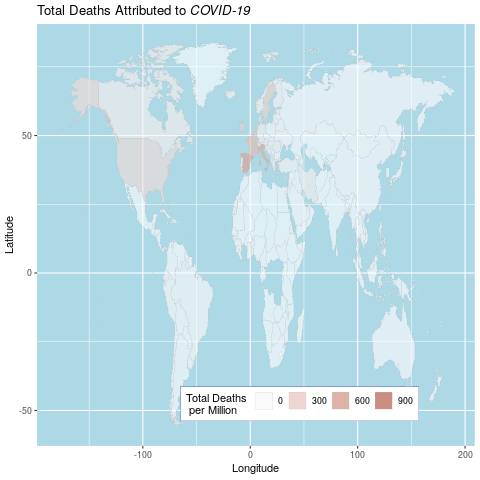
\includegraphics[width=.9\linewidth]{FirstChALL.png}
\caption{\label{fig:org7e64dfd}Chloropleth map of total deaths attributed to \emph{COVID-19} (per Million people)}
\end{figure}

\subsubsection{Europe Centric}
\label{sec:org70b837a}
The chloropleth map clearly shows that the disease has caused more fatalities
per capita in Europe and so the plot will be adjusted central to Europe.

As before it is necessary to rename the features of the dataset, however in this
instance small European countries such as Belgium should be retained (San marino
is a very small italian provice that isn't detectable in the visualisation and
skews the pallete, for this reason it will be removed), this is demonstrated in
figure \ref{orga5bd32f}

\begin{listing}[htbp]
\begin{minted}[]{r}
## Rename to facilitate joining with map
names(fatalprop) <- c("region", "total_deaths_per_million")

## San Marino will be shown by italy
 fatalprop <- fatalprop %>% filter(region!="San Marino")
\end{minted}
\caption{\label{orga5bd32f}Rename the features of the data and remove San Marino}
\end{listing}

In this map it will be desirable to have labels for the European countries
(whereas this would have made the worldwide map too busy), so this will be
implemented by using \texttt{dyplyr} to generate a second data set as shown in listing
\ref{org181dd8d} which can then be used to generate a plot with the \texttt{ggrepel} add on as shown in listing \ref{org8902b95}, this
produces the output shown in figure \ref{fig:org223d165}, for this plut bubbles were also implemented in order to help visualise the number of relative cases.
thee inspiration for the use of bubbles was the \emph{John Hopkins Coronavirus Dashboard} \cite{2020o} where a similar strategy was implemented to visualise the number of cases, a screenshot of this is provided in the appendix at figure \ref{fig:org615a27a}.

\begin{listing}[htbp]
\begin{minted}[]{r}
fatalmap <- left_join(fatalprop, some.eu.maps, by = "region")

## Filter out only Europe
fatalmap <-  fatalmap %>%
  filter(30 <  lat & lat < 65) %>%
  filter(-30 <  long & long < 35)

## Create Label Data Frame
region_lab_df <- fatalmap %>%
  dplyr::group_by(region) %>%
  dplyr::summarise(long = mean(long), lat = mean(lat)) %>%
   full_join(aggregate(total_deaths_per_million ~ region, fatalmap, mean))
\end{minted}
\caption{\label{org181dd8d}use \texttt{dplyr} to reduce the plot size and create a data frame of country labels}
\end{listing}

\begin{listing}[htbp]
\begin{minted}[]{r}
library(ggrepel)
ggplot(fatalmap, aes(map_id = region, label = region)) +
  geom_map(map = fatalmap,
           aes(fill = total_deaths_per_million),
           color = "white") +
  geom_point(data = region_lab_df, aes(y = lat, x = long, size = total_deaths_per_million), alpha = 0.45, colour = "blue", stroke = 1, fill = "white", shape = 21) +  scale_size_continuous(range = c(1, 25), name = "Total Number \n of Deaths") +
  guides(size = FALSE) +
  expand_limits(x = fatalmap$long, y = fatalmap$lat) +
  scale_fill_viridis_c(option = "C") +
  scale_fill_gradient(high = "darkred", low = "white") +
  guides(fill = guide_legend("Total Deaths \n per Million")) +
  # Change the colors of plot panel background to lightblue
  # and the color of grid lines to white
  theme(
    panel.background = element_rect(
      fill = "lightblue",
      colour = "lightblue",
      size = 0.5,
      linetype = "solid"
    ),
    legend.position = c(0.1, 0.6),
    legend.direction = "vertical",
    legend.background = element_rect(
      fill = "white",
      size =
        1.1,
      colour = "darkblue",
      linetype = "solid"
    )
  ) +
  labs(
    x = "Longitude",
    y = "Latitude",
    title = TeX("Total Deaths Attributed to \\textit{COVID-19}")
  ) +
  geom_text_repel(
    data = region_lab_df,
    aes(y = lat, x = long, label = region),
    size = 2,
    col = "black",
    nudge_y = 0.7,
    nudge_x = -0.5,
    min.segment.length = 0.6,
    force = 2
  )
\end{minted}
\caption{\label{org8902b95}Generate a Chloropleth map centred on Europe using \texttt{ggplot2}}
\end{listing}


\begin{figure}[htbp]
\centering
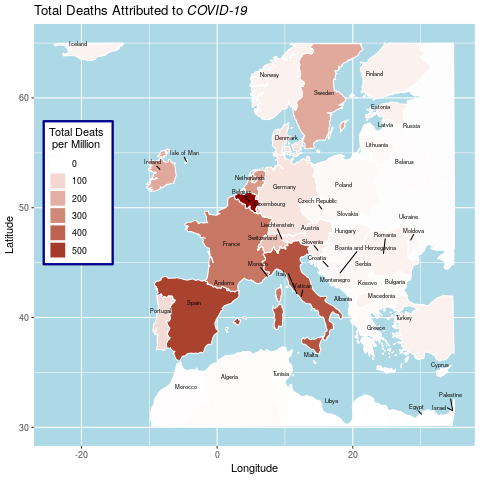
\includegraphics[width=10cm]{SecChEur.png}
\caption{\label{fig:org223d165}Europe Centred Chloropleth of Deaths Attributed to \emph{COVID-19}}
\end{figure}


\section{Time Series}
\label{sec:orgd18e079}
The spread of disease over time can often be modelled by exponential model as demonstrated in equations \eqref{exp1} and \eqref{exp2}, for this reason the use of a \$\(\log\)\$-scale will linearise trends and so the use of a \$\(\log\)\$-scale will make it easier to compare the rates of population change between different countries.



\begin{align}
  \frac{\mathrm{d} p}{\mathrm{d} t} \propto p &\implies p = Ce^{kt} \quad \exists k,c \in \mathbb{R} \label{exp1} \\
  \frac{\mathrm{d} p}{\mathrm{d} t} \propto p \wedge    \frac{\mathrm{d} p}{\mathrm{d} t} \propto (N-p) &\implies p = \frac{ke^{Nt}}{1-ke^{Nt}} \quad \exists k \in \mathbb{R}, N \in \mathbb{R^+} \label{exp1} \label{exp2}
\end{align}

In addition to a \(\log-\) scale, scaling the data to be relative to the number of days since the first case can allow the trends of the data to be compared, this was implemented by \emph{John Hopkins University} in a visualisation published in the \emph{Guardian} \cite{gutierrez2020}. \label{orgda7745e}

\subsection{Technical Details}
\label{sec:org190a922}

\subsection{Advantages compared to other methods}
\label{sec:orgd3a1d68}
\begin{itemize}
\item The advantage to a log-scaled plot is that it allows rates of change to be
compared between countries
\item Making the Data Relative to the day of the first infection allows individual
countries to be compared in terms of there response
\end{itemize}
\subsection{Disasadvantages}
\label{sec:org09b797c}
\begin{itemize}
\item A log-scaled plot can be misleading if it is not made clear, his particularly
true for readers who have limited mathematical training.
\begin{itemize}
\item For this reason a plot without log-scaling was included and the axis were
labelled accordingly
\end{itemize}
\item Making Data relative to the day of the first infection may not make clear that
certain countries had \emph{/forewarning} of the disease by virtue of the delay.
\end{itemize}
\subsection{Discussion on analysis results}
\label{sec:org32481c2}
\subsection{Discussion on other Aspects}
\label{sec:org5cd481d}
\subsection{Literature review of related work}
\label{sec:orgdb93e1d}
As mentioned in section \ref{orgda7745e} the use of the log-scaled and date-adjusted plot was implemented by \emph{John Hopkins University} in a visualisation published in \emph{The Guardian} newspaper \cite{gutierrez2020}.



\section{Bar Chart}
\label{sec:org574a540}

\section{Pie Chart}
\label{sec:org7a659d1}

\section{Spider Chart / Star Plot}
\label{sec:org1cd00da}

\section{Multiple Line Charts}
\label{sec:org086c831}

\section{Parallell Co-ordinates}
\label{sec:org246372d}
each line is a country
each column is a feature like testing, death and cases.

\href{https://stackoverflow.com/a/35206832/10593632}{This Stack Post shows how to make them curvy}

\section{3D Scatter Plot}
\label{sec:orgef591b1}
\section{Log Scaled from 100th case\hfill{}\textsc{ATTACH}}
\label{sec:orgb998fb8}
\begin{center}
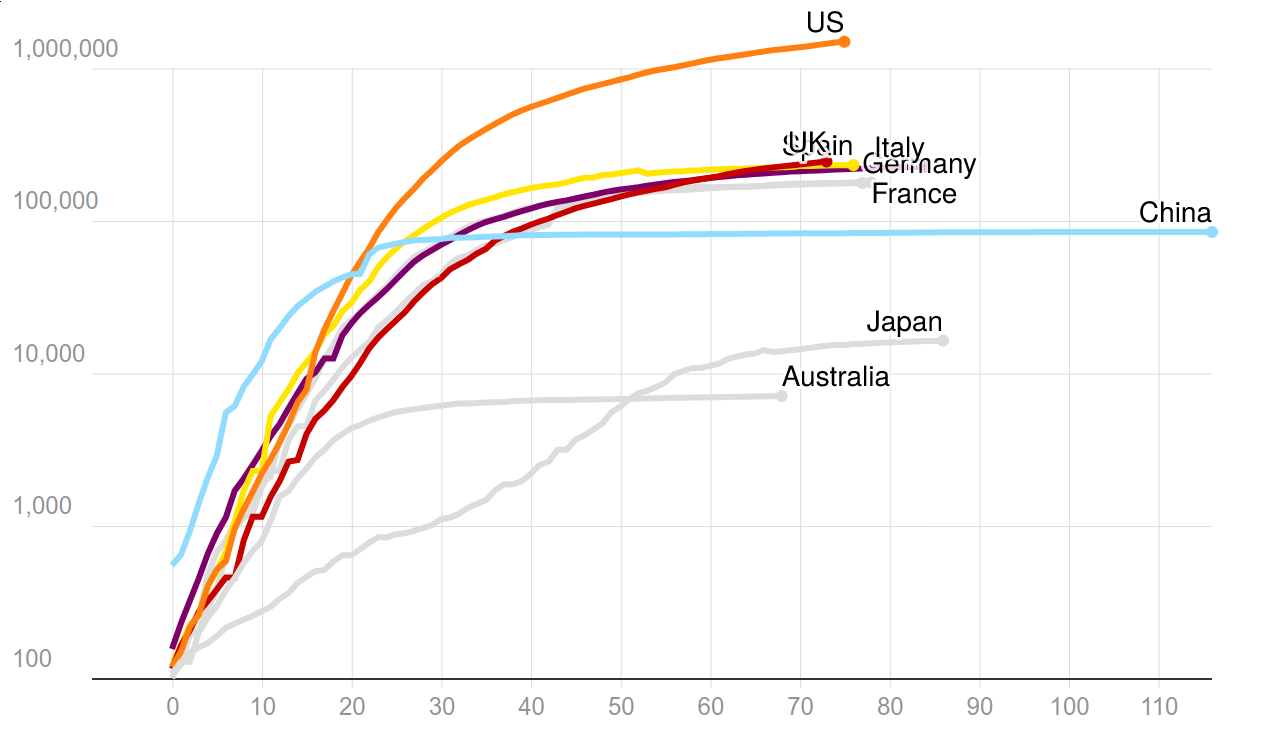
\includegraphics[width=.9\linewidth]{./_20200518_184546screenshot.png}
\end{center}

\section{Bubble Plot\hfill{}\textsc{ATTACH}}
\label{sec:org03453be}
\href{https://www.theguardian.com/world/2020/may/18/coronavirus-world-map-which-countries-have-the-most-cases-and-deaths}{Guardian}


\begin{center}
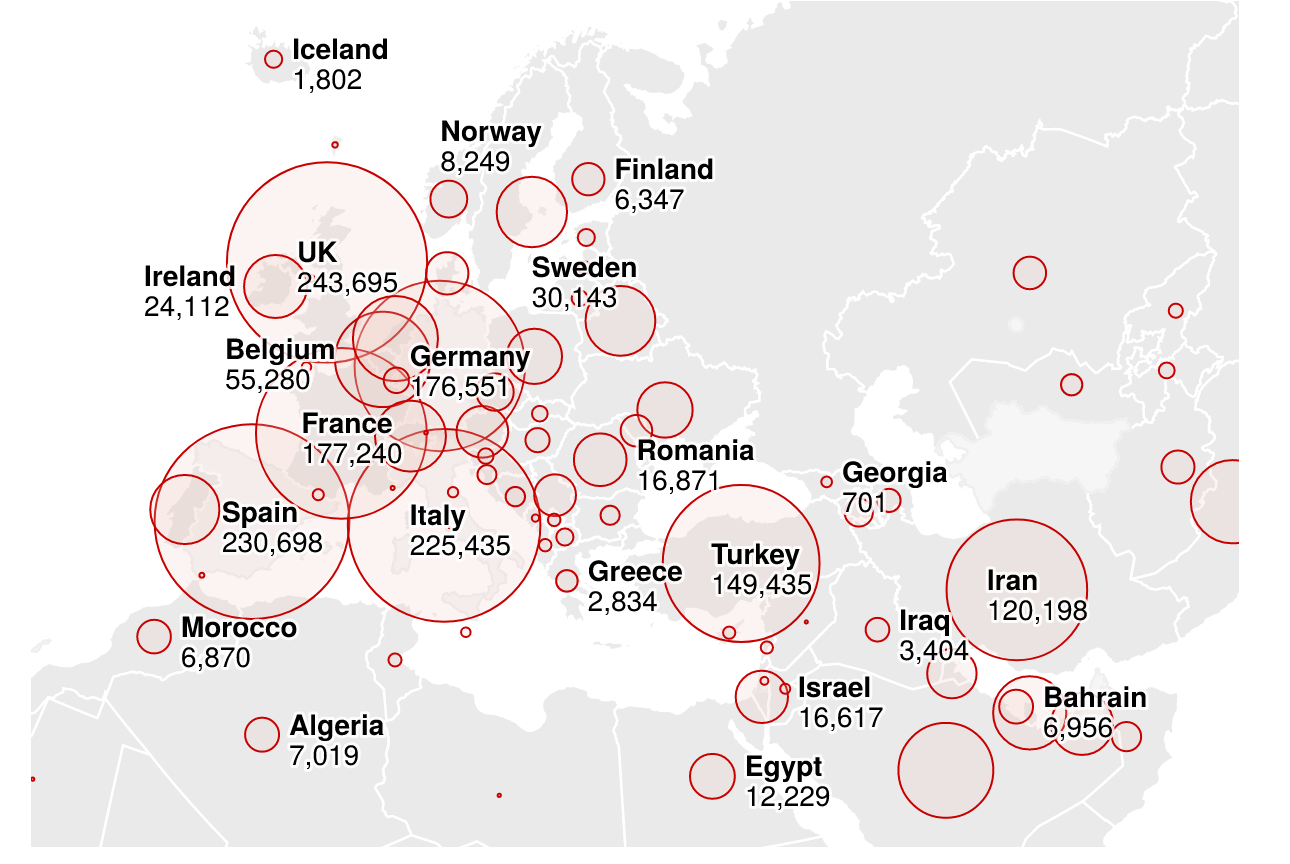
\includegraphics[width=10cm]{./_20200518_184850screenshot.png}
\end{center}




\section{Animation of 3d Chloropleth heatmap}
\label{sec:org0f605b9}

visualisation

The total number of deaths per country can be analysed using
\subsection{Technical Details}
\label{sec:orgda0a6ca}
\subsection{Advantages compared to other methods}
\label{sec:org62ec7d4}
\subsection{Disasadvantages}
\label{sec:orgd1d052a}
\subsection{Discussion on analysis results}
\label{sec:org6b274e8}
\subsection{Discussion on other Aspects}
\label{sec:org68719b3}
\subsection{Literature review of related work}
\label{sec:org99999c8}

\section{For Each Visualisation}
\label{sec:org51b751c}

\subsection{Technical Details}
\label{sec:orge59d4df}
\subsection{Advantages compared to other methods}
\label{sec:orgcf32daa}
\subsection{Disasadvantages}
\label{sec:org9c68d96}
\subsection{Discussion on analysis results}
\label{sec:org805633b}
\subsection{Discussion on other Aspects}
\label{sec:org2c67c23}
\subsection{Literature review of related work}
\label{sec:orgfc48c02}

\section{Apendix\hfill{}\textsc{ATTACH}}
\label{sec:org077d0b0}
\begin{figure}[htbp]
\centering
\includegraphics[width=.9\linewidth]{/home/ryan/Notes/Org/.attach/84/c19d03-8ab7-4793-a86d-e861e1bffe2b/_20200521_140312screenshot.png}
\caption{\label{fig:org615a27a}John Hopkins Bubble Chart \cite{2020o}}
\end{figure}

\section{References}
\label{sec:org2fdbae4}
\label{org89765da}
\bibliography{../../../../Studies/Papers/references}

\label{org655b7fa}
 \bibliographystyle{unsrt}
\end{document}
